\documentclass[11pt,a4paper]{article}

% ===================== Codificación y fuentes =====================
\usepackage[utf8]{inputenc}
\usepackage[T1]{fontenc}

% ===================== Página y utilidades ========================
\usepackage[left=2.5cm,right=2.5cm,top=2.5cm,bottom=2.5cm]{geometry}
\usepackage{array}
\usepackage{enumitem}
\usepackage{graphicx}
\usepackage{xcolor}
\usepackage{titlesec}
\usepackage{fancyhdr}
\usepackage[most]{tcolorbox}
\usepackage{hyperref}
\usepackage{booktabs}

% ===================== Etiquetas en español (sin babel) ===========
\renewcommand{\contentsname}{Índice}
\renewcommand{\figurename}{Figura}
\renewcommand{\tablename}{Tabla}
\renewcommand{\refname}{Bibliografía}

% ===================== Escala de grises (sin color) ================
\definecolor{negro}{RGB}{0,0,0}
\definecolor{gris}{RGB}{90,90,90}
\definecolor{grisclaro}{RGB}{150,150,150}
\definecolor{fillgray}{RGB}{175,175,175}

% ===================== Hipervínculos (negro) =======================
\hypersetup{colorlinks=true, linkcolor=negro, urlcolor=negro, citecolor=negro}

% ===================== Estilo de títulos ===========================
\titleformat{\section}{\large\bfseries\color{negro}}{\thesection.}{0.5em}{}
\titleformat{\subsection}{\normalsize\bfseries\color{negro}}{\thesubsection}{0.5em}{}
\titlespacing*{\section}{0pt}{1.4em}{0.4em}
\titlespacing*{\subsection}{0pt}{1.0em}{0.3em}

% ===================== Pie de página ===============================
\pagestyle{fancy}
\fancyhf{}
\fancyfoot[L]{\footnotesize\color{gris}Magíster en Ciencia de Datos e Inteligencia Artificial}
\fancyfoot[R]{\footnotesize\color{gris}\thepage}
\renewcommand{\headrulewidth}{0pt}
\renewcommand{\footrulewidth}{0.4pt}

% ===================== Comandos del docente ========================
\newcommand{\guia}[1]{{\small\itshape\color{gris}#1}\par\vspace{0.15em}}
\newcommand{\resp}{{\footnotesize\itshape\color{fillgray}[\,Desarrollen aquí\,]}\par\vspace{1.1em}}

% Caja de información de la evaluación (escala de grises):
\newtcolorbox{infobox}[1][Información de la evaluación]{colback=black!3,colframe=negro,
  fonttitle=\bfseries,coltitle=white,title={#1},boxrule=0.6pt,arc=1pt,
  left=8pt,right=8pt,top=6pt,bottom=6pt,breakable}

% Caja de conexión con evaluaciones previas (gris, sin color):
\newtcolorbox{conexionbox}[1][Conexión con evaluaciones anteriores]{colback=black!6,colframe=gris,
  fonttitle=\bfseries,coltitle=white,title={#1},boxrule=0.6pt,arc=1pt,
  left=8pt,right=8pt,top=6pt,bottom=6pt,breakable}

% ===================== Datos del grupo (COMPLETAR) ==================
\newcommand{\proyTitulo}{Predicción de riesgo de enfermedad coronaria a 10 años}
\newcommand{\proyIntegrantes}{Felipe Díaz Toro, Pablo Ríos Passteni, Guillermo Subiabre Chacón, Ninoska Yévenes Hernández}
\newcommand{\proyDataset}{Framingham Heart Study (Riesgo Cardiovascular)}
\newcommand{\proyDocente}{Jean Paul Maidana}
\newcommand{\proyFecha}{08/10/2026}
\newcommand{\proyRepo}{\url{https://github.com/fdiaztoro/proyecto-grupo3-mcdi501}}

\setlength{\parindent}{0pt}
\setlength{\parskip}{0.35em}

\begin{document}
\pagenumbering{gobble}

\thispagestyle{empty}
\begin{center}
\vspace*{1.0cm}

\includegraphics[height=4.4cm]{logo_unab.png}\\[1.3cm]

{\footnotesize\color{gris}\MakeUppercase{Magíster en Ciencia de Datos e Inteligencia Artificial}}\\[0.15cm]
{\footnotesize\color{grisclaro}MCDI501: Estadística Computacional para la Toma de Decisiones}\\[2.0cm]

{\Large\bfseries\color{negro} Evaluación Formativa 1}\\[0.45cm]
{\large\color{negro} Análisis Exploratorio e Inferencial (práctica)}\\[1.0cm]

{\small\itshape\color{gris} Informe individual o grupal \textperiodcentered\ 0\,\% (formativa)}
\end{center}

\vspace{1.6cm}

\begin{flushleft}
\setlength{\extrarowheight}{5pt}
\begin{tabular}{@{}>{\bfseries\color{negro}}l >{\raggedright\arraybackslash}p{11cm}@{}}
Título del proyecto: & \proyTitulo \\
Integrantes:         & \proyIntegrantes \\
Dataset:             & \proyDataset \\
Docente:             & \proyDocente \\
Fecha:               & \proyFecha \\
Repositorio GitHub:  & \proyRepo \\
\end{tabular}
\end{flushleft}

\clearpage
\pagenumbering{arabic}
\begin{infobox}
\textbf{Fase del proyecto:} Fase 2: Búsqueda y recopilación de información\\
\textbf{Modalidad:} Grupal\qquad\textbf{Ponderación:} 0\,\% (formativa)\\
\textbf{Entregable:} Informe en formato PDF, subido a Canvas\\
\textbf{Resultado de aprendizaje (RA1):} aplicar conceptos fundamentales de probabilidad e inferencia estadística en la resolución de problemas de decisión bajo incertidumbre.\\
\textbf{Indicadores:} ID1.2, ID1.3, ID1.4.
\end{infobox}

\vspace{0.5em}
\tableofcontents
\newpage

\section{Introducción}
\guia{Presenten brevemente el conjunto de datos definido por el equipo en la fase anterior del proyecto y el propósito de este informe de avance.}

Para esta fase se trabajó con el dataset \textbf{Framingham Heart Study} (riesgo cardiovascular), la
versión pública publicada en Kaggle (\textit{Heart Disease Prediction using Logistic Regression}) de
uno de los estudios cardiovasculares longitudinales más citados en la literatura médica. Reúne
información de \textbf{4.238 participantes} de la ciudad de Framingham (Massachusetts, EE.\,UU.), cada
uno descrito por 15 variables medidas al inicio del seguimiento, e indica si la persona desarrolló
\textbf{enfermedad coronaria (CHD) en los diez años siguientes}. Esa es la variable objetivo,
\texttt{TenYearCHD}.

En salud pública y atención primaria, anticiparse al riesgo cardiovascular permite priorizar
controles y prevención antes de que la enfermedad se manifieste. Pero la decisión se toma bajo
incertidumbre: solo se observa una muestra de personas, y las asociaciones entre los factores de
riesgo y el desenlace son, como se verá, débiles a moderadas. Este informe de avance es una primera
caracterización estadística del conjunto. Incluye estadística descriptiva, estimación por
intervalos de confianza y pruebas de hipótesis, y deja sentadas las bases del modelamiento
posterior. Los cálculos usan la semilla \texttt{42} y están documentados en el cuaderno adjunto
(\texttt{Formativa1\_FraminghamHeartStudy\_Codigo.ipynb}).

\section{Aplicación de estadística descriptiva}
\guia{(15 pts, ID1.2) Caractericen las variables del conjunto de datos mediante medidas de tendencia central, dispersión y representaciones gráficas adecuadas a cada tipo de variable.}

\subsection{Tipos de variables y medidas resumen}
El conjunto tiene 16 variables: el objetivo binario (\texttt{TenYearCHD}), seis indicadores binarios
(sexo, fumador actual, medicación antihipertensiva, ACV previo, hipertensión prevalente y diabetes),
una variable ordinal (nivel educativo, 1 a 4), un conteo (cigarrillos por día) y siete variables
numéricas continuas o cuasi-continuas (edad, colesterol total, presión sistólica y diastólica,
índice de masa corporal, frecuencia cardíaca y glucosa). Predominan las variables binarias, por lo
que su media se interpreta como una proporción. La Tabla~\ref{tab:descriptivos} resume la tendencia
central y la dispersión de las variables numéricas.

\begin{table}[htbp]
\centering
\caption{Medidas descriptivas de las variables numéricas (calculadas con los datos disponibles de cada variable).}
\label{tab:descriptivos}
\begin{tabular}{lrrrrr}
\toprule
\textbf{Variable} & \textbf{Media} & \textbf{Mediana} & \textbf{Desv. est.} & \textbf{Mínimo} & \textbf{Máximo} \\
\midrule
Edad (años)                  & 49{,}58  & 49{,}00  & 8{,}57  & 32    & 70  \\
Cigarrillos por día          & 9{,}00   & 0{,}00   & 11{,}92 & 0     & 70  \\
Colesterol total (mg/dL)     & 236{,}72 & 234{,}00 & 44{,}59 & 107   & 696 \\
Presión sistólica (mmHg)     & 132{,}35 & 128{,}00 & 22{,}04 & 83{,}5  & 295 \\
Presión diastólica (mmHg)    & 82{,}89  & 82{,}00  & 11{,}91 & 48    & 142{,}5 \\
Índice de masa corporal      & 25{,}80  & 25{,}40  & 4{,}08  & 15{,}54 & 56{,}8 \\
Frecuencia cardíaca          & 75{,}88  & 75{,}00  & 12{,}03 & 44    & 143 \\
Glucosa (mg/dL)               & 81{,}97  & 78{,}00  & 23{,}96 & 40    & 394 \\
\bottomrule
\end{tabular}
\end{table}

La edad es aproximadamente simétrica (media 49{,}6 y mediana 49{,}0 años; rango de 32 a 70). El
colesterol total, la presión sistólica y la glucosa tienen la media por sobre la mediana (236{,}7 vs.\
234{,}0; 132{,}4 vs.\ 128{,}0; 82{,}0 vs.\ 78{,}0) y máximos muy alejados del resto (696 mg/dL, 295 mmHg y
394 mg/dL), señal de asimetría a la derecha y de valores extremos. En cigarrillos por día la
mediana es 0 y la media 9{,}0: más de la mitad de los participantes no fuma, y la media la elevan
los fumadores intensos (hasta 70 cigarrillos diarios).

\begin{table}[htbp]
\centering
\caption{Dispersión y forma de las variables numéricas.}
\label{tab:dispersion}
\begin{tabular}{lrrr}
\toprule
\textbf{Variable} & \textbf{IQR} & \textbf{CV (\%)} & \textbf{Asimetría} \\
\midrule
Edad (años)               & 14{,}00 & 17{,}29  & 0{,}23 \\
Cigarrillos por día       & 20{,}00 & 132{,}40 & 1{,}25 \\
Colesterol total (mg/dL)  & 57{,}00 & 18{,}84  & 0{,}87 \\
Presión sistólica (mmHg)  & 27{,}00 & 16{,}65  & 1{,}15 \\
Presión diastólica (mmHg) & 14{,}88 & 14{,}37  & 0{,}71 \\
Índice de masa corporal   & 4{,}97  & 15{,}81  & 0{,}98 \\
Frecuencia cardíaca       & 15{,}00 & 15{,}85  & 0{,}64 \\
Glucosa (mg/dL)           & 16{,}00 & 29{,}23  & 6{,}21 \\
\bottomrule
\end{tabular}
\end{table}

La edad es la variable más simétrica (asimetría 0{,}23) y la glucosa la más sesgada (6{,}21), arrastrada
por valores extremos. El colesterol, la presión sistólica y el IMC muestran asimetría moderada a la
derecha, lo que respalda usar la mediana como referencia. Los cigarrillos por día tienen el mayor
coeficiente de variación (132\,\%): muchas personas no fuman y unas pocas fuman mucho.

\begin{table}[htbp]
\centering
\caption{Variables binarias y tasa de CHD a 10 años según el atributo.}
\label{tab:binarias}
\begin{tabular}{lrrr}
\toprule
\textbf{Variable} & \textbf{\% con atributo} & \textbf{\% CHD con atributo} & \textbf{\% CHD sin atributo} \\
\midrule
Sexo masculino                & 42{,}9 & 18{,}9 & 12{,}4 \\
Fumador actual                & 49{,}4 & 15{,}9 & 14{,}5 \\
Medicación antihipertensiva   & 3{,}0  & 33{,}1 & 14{,}6 \\
ACV previo                    & 0{,}6  & 44{,}0 & 15{,}0 \\
Hipertensión prevalente       & 31{,}1 & 24{,}7 & 10{,}9 \\
Diabetes                      & 2{,}6  & 36{,}7 & 14{,}6 \\
\bottomrule
\end{tabular}
\end{table}

La tasa de CHD es mayor en quienes tienen cada antecedente (ACV previo, diabetes, medicación
antihipertensiva, hipertensión y sexo masculino), mientras que fumar actualmente casi no cambia la
tasa (15{,}9\,\% vs.\ 14{,}5\,\%). Son comparaciones descriptivas, sin ajustar por edad ni otras
variables, y los grupos con ACV previo (unas 25 personas) o diabetes son pequeños, por lo que esas
tasas son menos precisas. El nivel educativo se distribuye así entre los casos válidos: 41{,}6\,\% nivel 1,
30{,}3\,\% nivel 2, 16{,}6\,\% nivel 3 y 11{,}4\,\% nivel 4.

\subsection{Calidad de datos}
El 15{,}2\,\% de los participantes (644 de 4.238) desarrolló enfermedad coronaria en diez años, es
decir, unos 5{,}6 personas sanas por cada caso: el objetivo está desbalanceado. No hay filas
duplicadas. Hay datos faltantes en siete variables; la glucosa concentra la mayor parte (388
registros, 9{,}2\,\%), seguida del nivel educativo (105, 2{,}5\,\%), y 582 filas (13{,}7\,\%) tienen al
menos un dato faltante, que es lo que se perdería al eliminar filas incompletas. Los valores
extremos según la regla de Tukey van de 1{,}3\,\% (colesterol) a 4{,}9\,\% (glucosa) de las
observaciones. No hay inconsistencias entre variables relacionadas: ninguna presión diastólica supera a la sistólica y el hábito de fumar es coherente con los cigarrillos por día.

\begin{figure}[htbp]
\centering
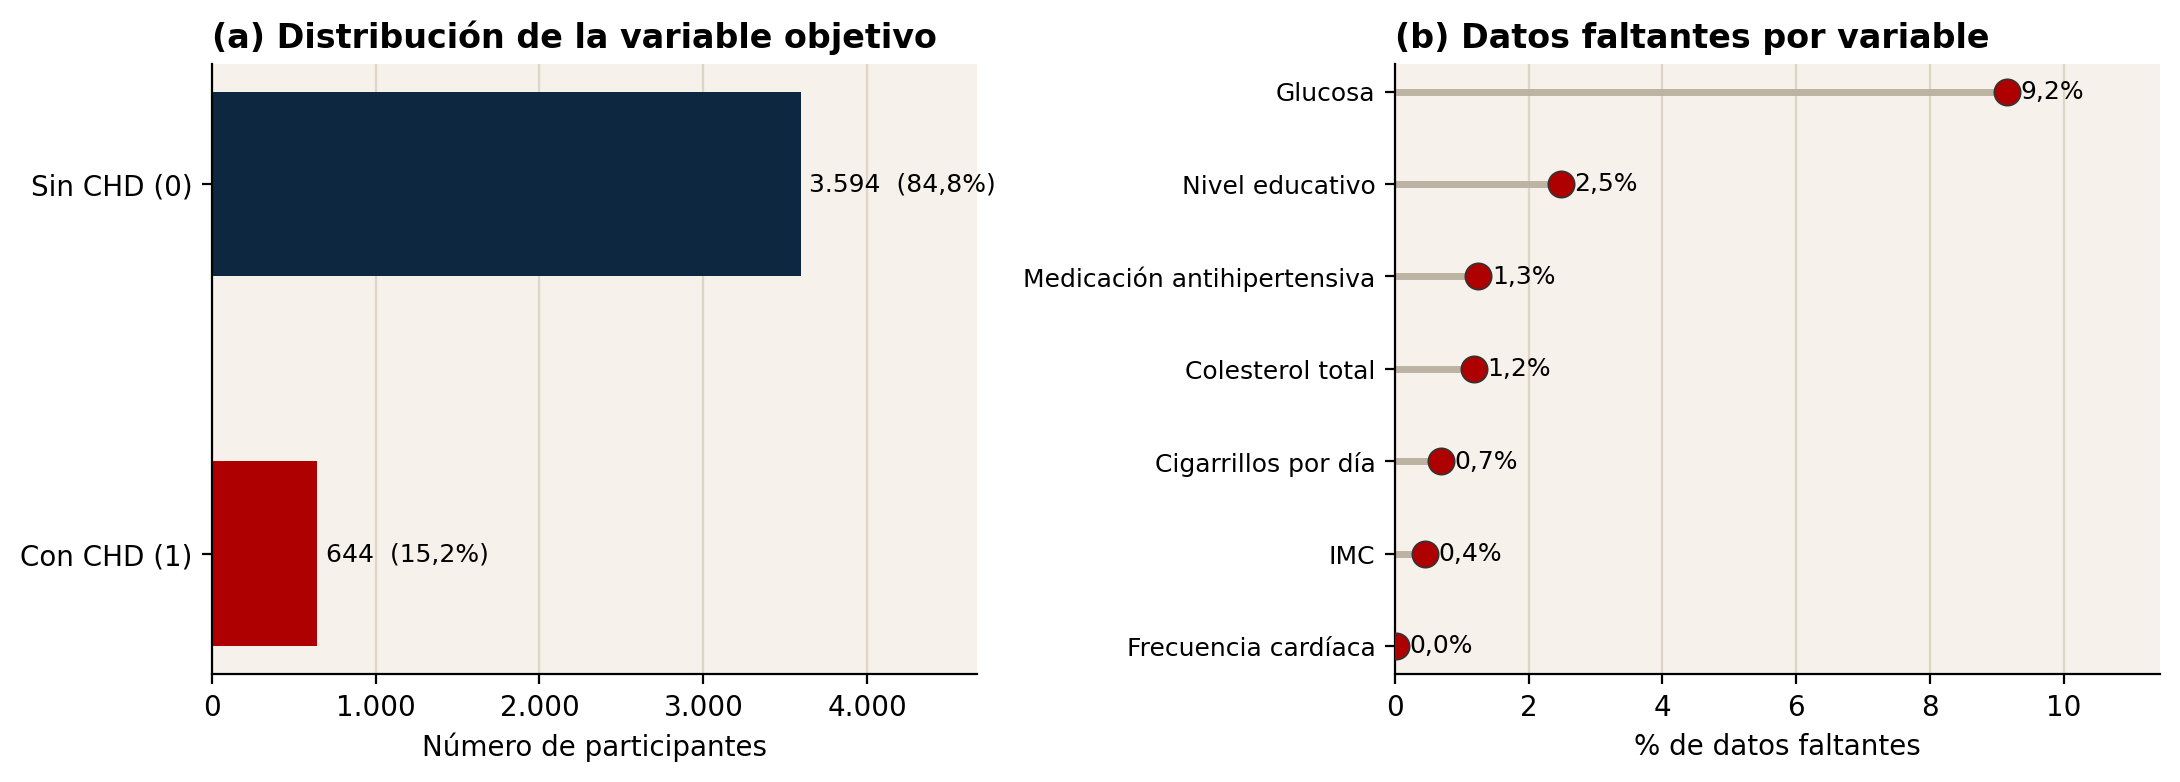
\includegraphics[width=\linewidth]{figuras/fig_panorama.png}
\caption{(a) Distribución de la variable objetivo. (b) Porcentaje de datos faltantes por variable.}
\label{fig:panorama}
\end{figure}

El panel (a) de la Figura~\ref{fig:panorama} muestra el desbalance de la variable objetivo: la
exactitud global sería engañosa (predecir siempre ``sin CHD'' acertaría 84{,}8\,\%), por lo que habrá
que evaluar los modelos futuros con métricas sensibles a la clase minoritaria. El panel (b) muestra
que los faltantes son pocos salvo en la glucosa (9{,}2\,\%) y la educación (2{,}5\,\%); el resto no
supera el 1{,}3\,\%.

\begin{figure}[htbp]
\centering
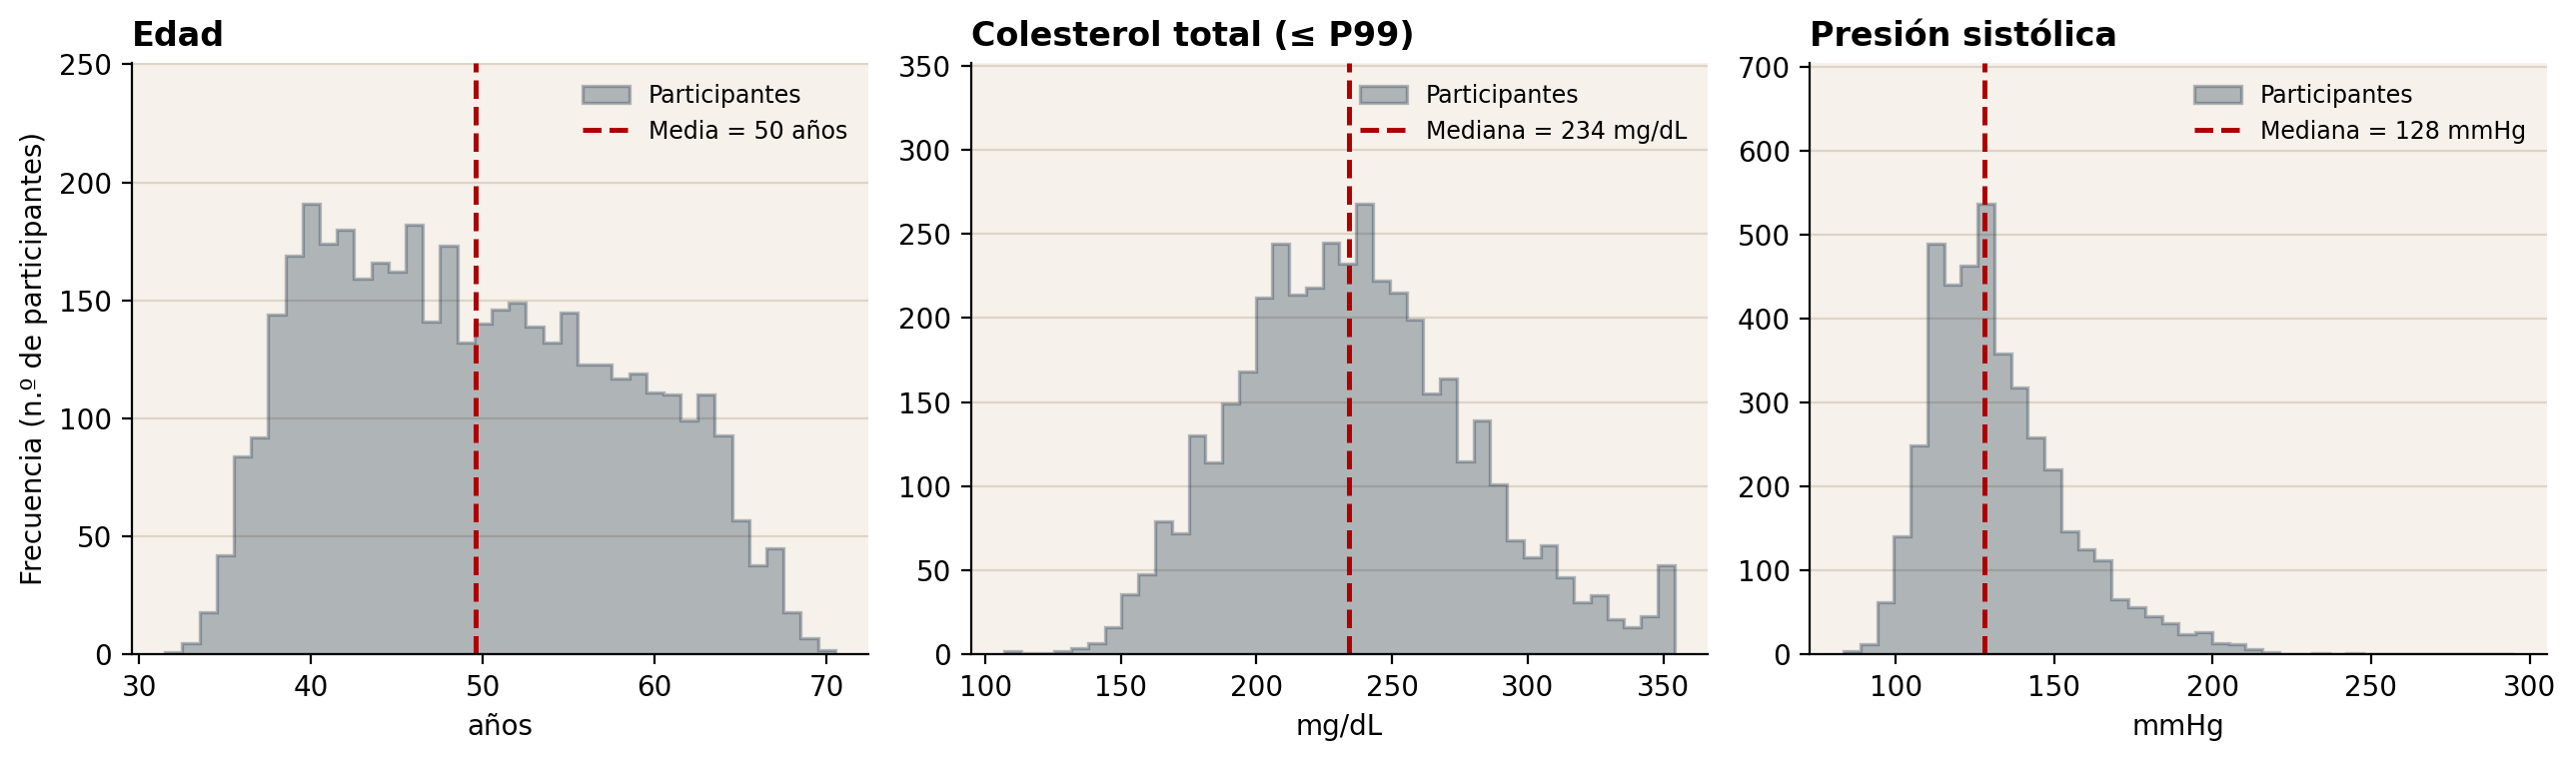
\includegraphics[width=\linewidth]{figuras/fig_distribuciones.png}
\caption{Distribución de tres variables cuantitativas representativas, con su media o mediana de referencia.}
\label{fig:distribuciones}
\end{figure}

La Figura~\ref{fig:distribuciones} confirma estas formas: la edad se distribuye de manera
aproximadamente simétrica en torno a los 50 años; el colesterol total y la presión sistólica son
asimétricos a la derecha, con la mediana (234 mg/dL y 128 mmHg) por debajo de la media y una cola de
valores altos. Por eso en esas dos variables se usa la mediana como referencia, y el colesterol se
recorta al percentil 99 solo para efectos de visualización (los cálculos usan todos los datos).

\begin{figure}[htbp]
\centering
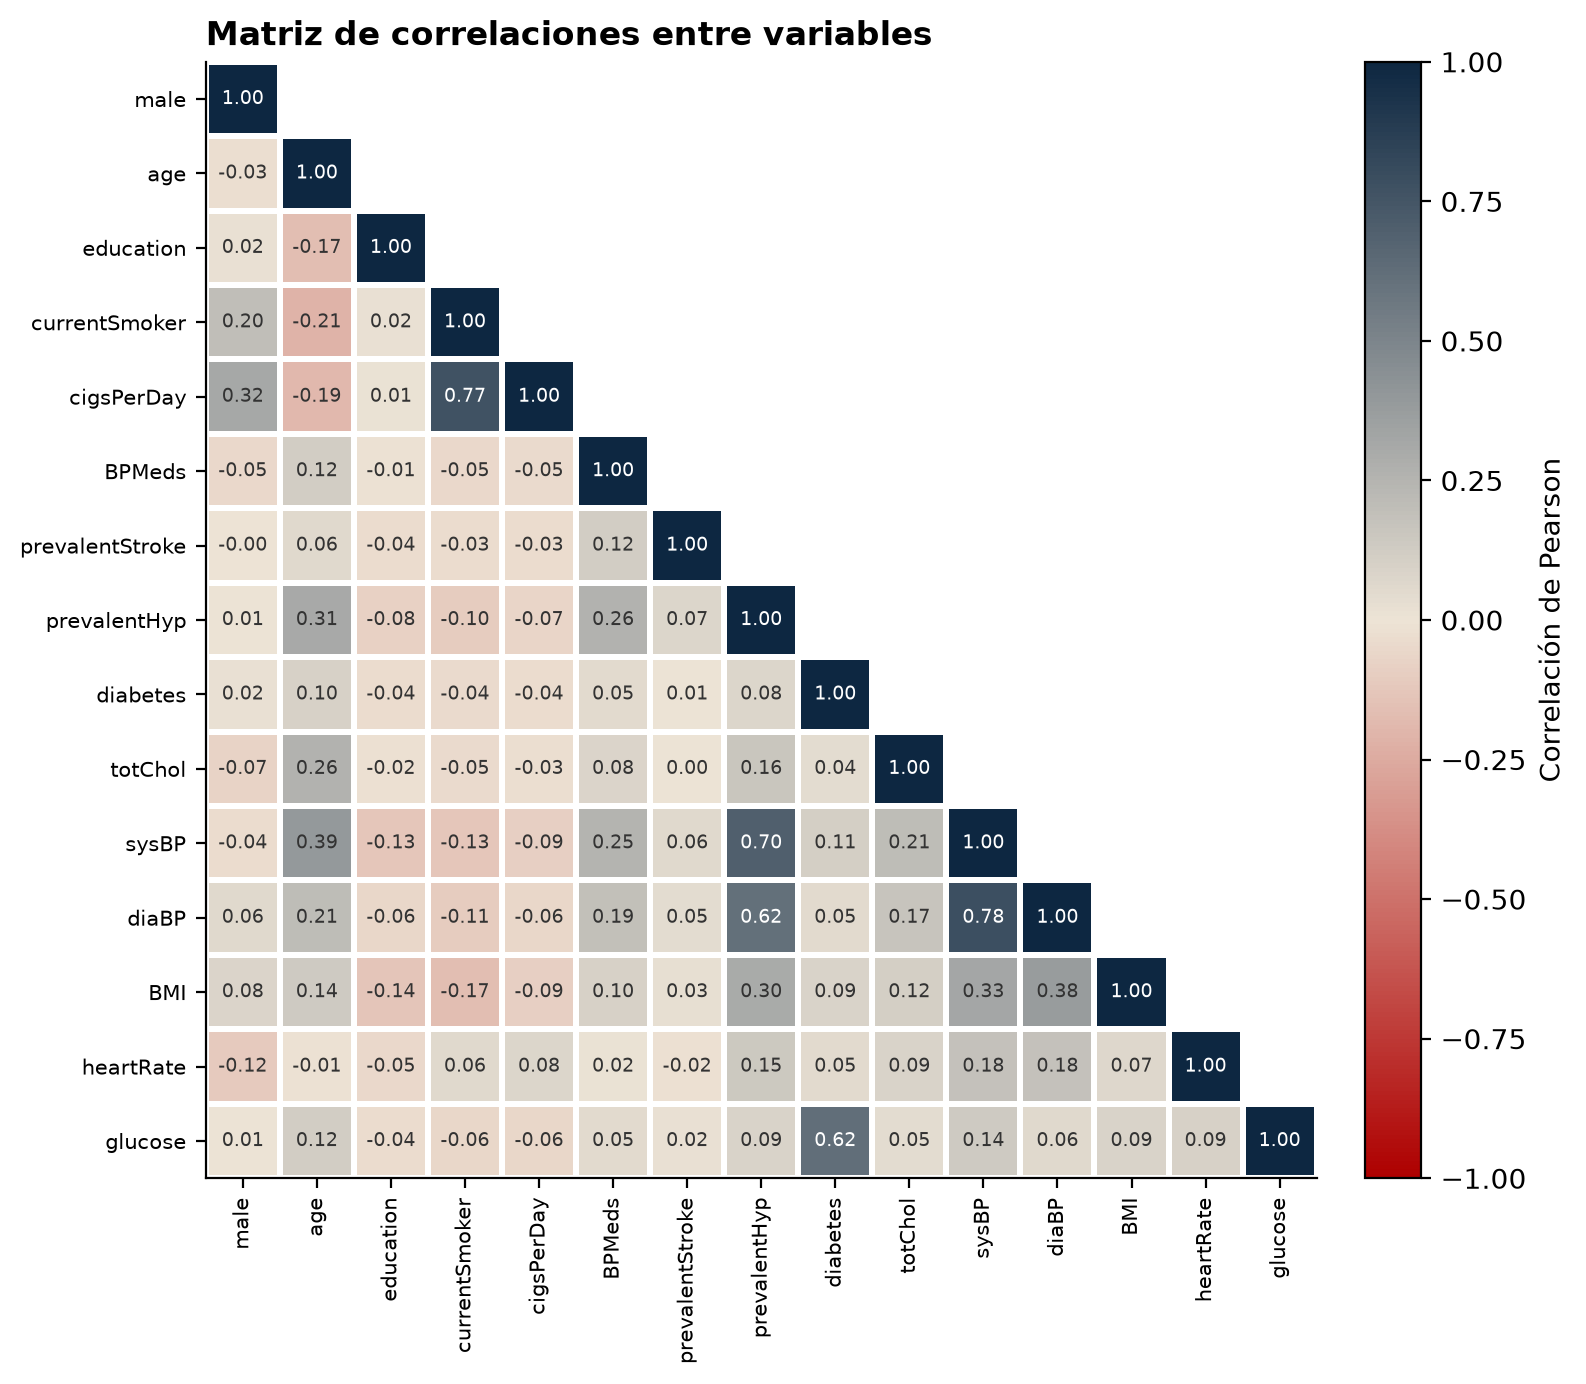
\includegraphics[width=0.85\linewidth]{figuras/fig_correlacion.png}
\caption{Matriz de correlaciones entre las variables predictoras (triángulo inferior).}
\label{fig:correlacion}
\end{figure}

La matriz de correlaciones (Figura~\ref{fig:correlacion}) muestra que las correlaciones más altas
son entre presión sistólica y diastólica ($r=0{,}78$), fumador actual y cigarrillos por día
($r=0{,}77$, relación en parte estructural: quien no fuma tiene 0 cigarrillos), hipertensión
prevalente y presión sistólica ($r=0{,}70$), y diabetes y glucosa ($r=0{,}62$). El resto de las
correlaciones son débiles a moderadas. Al revisar la correlación de cada variable con el objetivo,
la edad ($r=0{,}23$) y la presión sistólica ($r=0{,}22$) son las que más se asocian linealmente con el
riesgo de CHD; el fumar y la frecuencia cardíaca son las más débiles ($r<0{,}03$).

\section{Estimación puntual e intervalos de confianza}
\guia{(15 pts, ID1.3) Utilicen métodos de estimación puntual e intervalos de confianza para determinar parámetros poblacionales relevantes del conjunto de datos, interpretando los resultados.}

Se estimaron tres parámetros poblacionales con un nivel de confianza del 95\,\%, usando la
aproximación normal que justifica el Teorema Central del Límite: $\bar{x} \pm z_{0{,}975}\cdot EE$,
con $EE = s/\sqrt{n}$ para las medias, y $\hat{p} \pm z_{0{,}975}\cdot\sqrt{\hat{p}(1-\hat{p})/n}$
para la proporción. La Tabla~\ref{tab:ic} resume los valores.

\begin{table}[htbp]
\centering
\caption{Estimación puntual e intervalos de confianza al 95\,\%.}
\label{tab:ic}
\begin{tabular}{lrrr}
\toprule
\textbf{Parámetro} & \textbf{Estimación} & \textbf{IC 95\,\%} & \textbf{$n$} \\
\midrule
Edad media (años)                & 49{,}58  & [49{,}33; 49{,}84]   & 4.238 \\
Colesterol total medio (mg/dL)   & 236{,}72 & [235{,}37; 238{,}07] & 4.188 \\
Proporción de CHD a 10 años      & 15{,}20\,\% & [14{,}12\,\%; 16{,}28\,\%] & 4.238 \\
\bottomrule
\end{tabular}
\end{table}

\textbf{Interpretación.} Con 4.238 participantes, el Teorema Central del Límite respalda la
aproximación normal en los tres casos, y los intervalos salen angostos por el tamaño de la
muestra. Con un 95\,\% de confianza, la edad media poblacional está entre 49{,}33 y 49{,}84 años, y la
proporción de personas que desarrollan CHD a 10 años cae entre 14{,}12\,\% y 16{,}28\,\%. El colesterol
total medio (236{,}72 mg/dL) se estimó con 50 observaciones menos por datos faltantes ($n=4.188$),
pero como representan solo 1{,}2\,\% del total, el intervalo [235{,}37; 238{,}07] sigue siendo confiable. Los intervalos usan los casos disponibles de cada variable, sin imputar. Como se vio en la sección anterior, el colesterol es asimétrico a la derecha; el Teorema Central
del Límite respalda que la \textit{media muestral} se distribuya de forma aproximadamente normal
pese a eso, así que el intervalo es válido, pero conviene recordar que la mediana (234{,}0 mg/dL)
sigue siendo la referencia más representativa del participante típico.

\section{Aplicación de una prueba de hipótesis}
\guia{(15 pts, ID1.4) Apliquen al menos una prueba de hipótesis básica, seleccionando el procedimiento adecuado según el tipo de variable y el nivel de significancia definido.}

Se aplicaron dos pruebas con un nivel de significancia $\alpha = 0{,}05$, eligiendo en cada caso el
procedimiento adecuado al tipo de variable involucrada.

\subsection{Prueba \textit{t} de Welch: edad entre quienes desarrollan CHD y quienes no}
Se compara la edad (variable continua) entre dos grupos independientes de tamaños muy distintos (644 y 3.594). Se usa la prueba \textit{t} de Welch porque no exige varianzas iguales; aquí son parecidas (64{,}1 y 70{,}8), por lo que el resultado coincide con el de Student:
$$H_0:\ \mu_{\text{CHD}} = \mu_{\text{no CHD}} \qquad \text{vs.} \qquad H_1:\ \mu_{\text{CHD}} \neq \mu_{\text{no CHD}}$$

Las medias muestrales son 54{,}15 años entre quienes desarrollan CHD ($n=644$) y 48{,}77 años entre
quienes no ($n=3.594$), una diferencia de casi 5{,}4 años. El estadístico da $t=15{,}58$ con un valor
$p<0{,}0001$, de modo que \textbf{se rechaza $H_0$}. El tamaño del efecto ($d$ de Cohen $=0{,}64$) es
moderado a grande: la edad separa razonablemente bien a ambos grupos, consistente con que fue la
variable con mayor correlación con el objetivo ($r=0{,}23$) en la sección anterior.

\subsection{Prueba \texorpdfstring{$\chi^2$}{chi-cuadrado} de independencia: hipertensión prevalente y CHD}
Se contrasta la independencia entre dos variables binarias, por lo que corresponde la prueba
$\chi^2$ de independencia sobre una tabla de $2\times2$:
$$H_0:\ \text{hipertensión prevalente y CHD son independientes} \qquad \text{vs.} \qquad H_1:\ \text{están asociadas}$$

La frecuencia esperada mínima es 200, muy por encima del umbral de 5, así que el supuesto de la
prueba se cumple. La asociación es significativa ($\chi^2=132{,}6$; $\text{gl}=1$; $p<0{,}0001$; sin corrección de continuidad, $\chi^2=133{,}7$, mismo resultado), con una intensidad débil a moderada ($V$ de Cramér $=0{,}18$).

\begin{figure}[htbp]
\centering
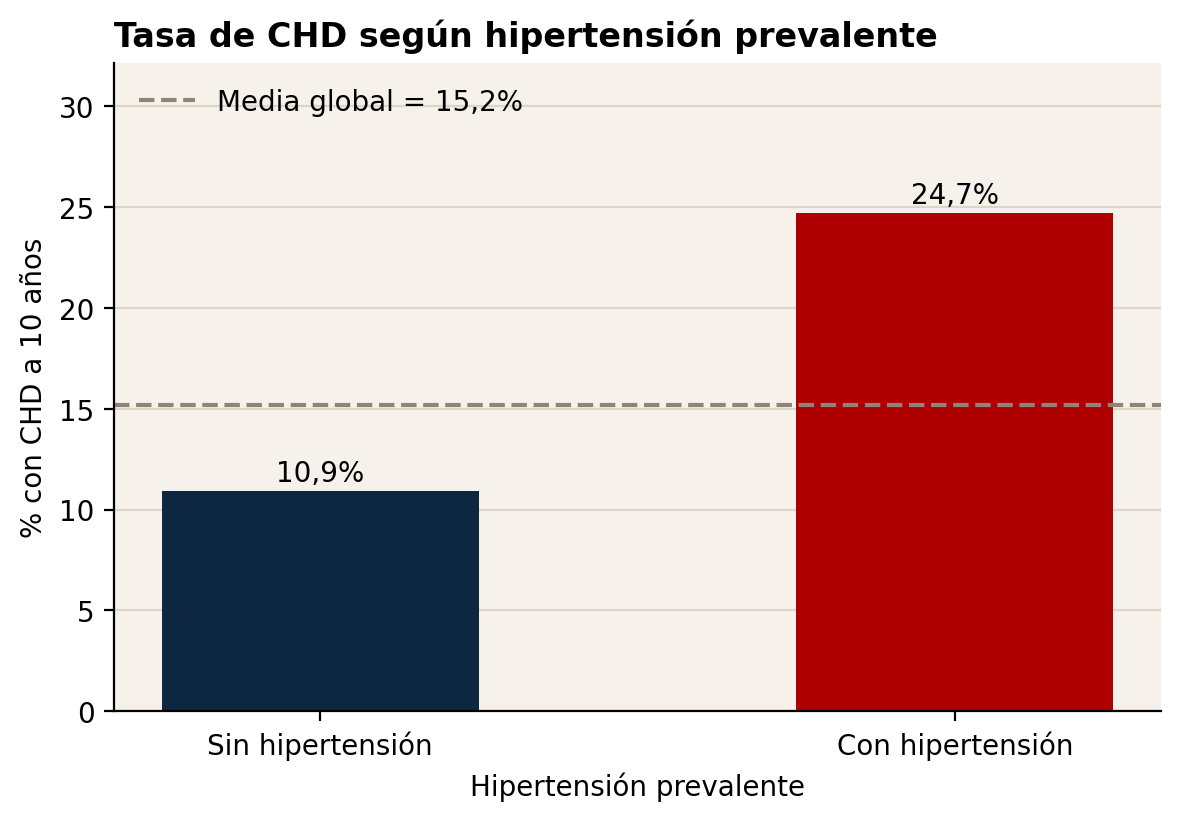
\includegraphics[width=0.75\linewidth]{figuras/fig_hipertension.png}
\caption{Tasa de CHD a 10 años según hipertensión prevalente, con la media global de referencia.}
\label{fig:hipertension}
\end{figure}

Como muestra la Figura~\ref{fig:hipertension}, el 24{,}7\,\% de quienes tienen hipertensión
prevalente desarrolla CHD a 10 años, frente al 10{,}9\,\% de quienes no la tienen: un \textbf{riesgo relativo de 2{,}26} (alrededor de 2{,}3 veces). En términos de correlación, la asociación con la hipertensión ($r=0{,}18$) es algo menor que la de la edad ($r=0{,}23$).

\section{Documentación de procedimientos y resultados}
\guia{(15 pts) Documenten de forma clara, ordenada y completa los procedimientos estadísticos aplicados y los resultados obtenidos, de manera que el análisis sea trazable.}

Todo el análisis se hizo en Python, con \texttt{pandas}, \texttt{numpy}, \texttt{scipy} y
\texttt{matplotlib}, y es reproducible fijando la semilla \texttt{42}. El cuaderno adjunto
(\texttt{Formativa1\_FraminghamHeartStudy\_Codigo.ipynb}) contiene el código completo, organizado en
los mismos bloques de este informe, y genera las figuras aquí incluidas. Los procedimientos
fueron:

\begin{itemize}[leftmargin=1.4em]
  \item \textbf{Descriptiva:} medidas de tendencia central y dispersión con \texttt{describe()} (más rango intercuartílico, coeficiente de variación y asimetría), regla de Tukey para valores extremos,
  clasificación de variables por tipo, y gráficos según el tipo de variable (barras para el
  objetivo, puntos para los faltantes, histogramas para las variables continuas y un mapa de calor
  para las correlaciones).
  \item \textbf{Estimación:} intervalos de confianza para las medias mediante
  $\bar{x}\pm z_{0{,}975}\cdot EE$, con $EE=s/\sqrt{n}$, y para la proporción mediante la
  aproximación normal (método de Wald).
  \item \textbf{Prueba de hipótesis:} \textit{t} de Welch (\texttt{scipy.stats.ttest\_ind},
  \texttt{equal\_var=False}) y prueba $\chi^2$ de independencia
  (\texttt{scipy.stats.chi2\_contingency}), ambas con $\alpha=0{,}05$; como medidas de efecto se usaron la $d$ de Cohen, la $V$ de Cramér y el riesgo relativo.
\end{itemize}

\section{Interpretación preliminar de resultados}
\guia{(15 pts) Presenten interpretaciones preliminares claras y coherentes, vinculando los resultados obtenidos con el problema de decisión bajo incertidumbre.}

De lo anterior se desprenden varias lecturas para el problema de anticipar riesgo cardiovascular.
La más clara tiene que ver con la \textbf{hipertensión prevalente}: quienes la tienen más que duplican su riesgo de desarrollar CHD a 10 años (riesgo relativo de 2{,}26), una señal fuerte y clínicamente relevante. La \textbf{edad} aporta otra señal, de tamaño moderado y también significativa ($d=0{,}64$): los pacientes mayores presentan más riesgo. En cambio, variables como el
hábito de fumar o la frecuencia cardíaca muestran una asociación lineal casi nula con el objetivo
($r<0{,}03$), lo que sugiere que, al menos de forma aislada, pesan menos que el historial de presión
arterial o la edad a la hora de estratificar el riesgo.

Quedan dos advertencias para las fases siguientes. El desbalance del objetivo (15{,}2\,\% con CHD)
obliga a evaluar los futuros modelos con métricas sensibles a la clase minoritaria, y no solo con
la exactitud global. Y la correlación moderada-alta entre hipertensión prevalente y presión
sistólica ($r=0{,}70$) desaconseja incluir ambas variables sin más en un modelo, por el riesgo de
colinealidad. Son hipótesis de trabajo; las evaluaciones posteriores dirán si se sostienen.

Los datos son observacionales, por lo que las asociaciones encontradas no implican causalidad. Con la información disponible, en atención primaria convendría priorizar el tamizaje y seguimiento de personas de mayor edad y con hipertensión, que concentran más casos de CHD a 10 años, con la salvedad de que ninguna variable por sí sola discrimina bien el riesgo.

\section{Presentación formal del informe}
\guia{(15 pts) Verifiquen redacción formal, uso adecuado de lenguaje estadístico y cumplimiento del formato solicitado antes de subir el PDF a Canvas.}

Este informe se redactó en un registro formal, con uso preciso de lenguaje estadístico
(estimación puntual, intervalo de confianza, valor $p$, nivel de significancia, tamaño del
efecto) y siguiendo la estructura de la plantilla solicitada. Antes de la entrega final, el
equipo verificó que los datos del encabezado (integrantes, docente, fecha y repositorio) estén
completos, que las figuras y tablas se referencien correctamente en el texto, y que el documento
se exporte en formato PDF para su carga en Canvas.

\end{document}
